\documentclass[11pt]{article}
%*******************************************************************
%--Packages
%*******************************************************************
\usepackage[final]{graphicx,epsfig}
\usepackage{subfigure}
\usepackage{subfigmat}
\usepackage{color}

\definecolor{red}{rgb}{1.0,0.0,0.0}
\setlength{\parindent}{0pt}
\setlength{\parskip}{5pt plus 2pt minus 1 pt}
\topmargin  -5mm
\evensidemargin 8mm
\oddsidemargin  2mm
\textwidth  158mm
\textheight 230mm
%\renewcommand{\baselinestretch}{1.0}
\frenchspacing
\sloppy

%%%%%%%%%%%%%%%%%%%%%%%%%%%%%%%%%%%%%%%%%%%%%%%%%%%%%%%%%%%%%%%%%%%%%%%

\begin{document}
\pagestyle{empty}

\begin{center}
  {\fontsize{14}{20}\bf 
    User-manual for COOLFluiD Finite Volume Inductively Coupled Plasma \\
    (version 2011.04) \\[10pt]}
\end{center}

\begin{center}
  {Nad\`{e}ge Villedieu, \underline{villedie@vki.ac.be} \\
    Von Karman Institute, Aeronautics \& Aerospace Dept.}
\end{center}

The test case for simulating the jet flow around a probe in Plasmatron testing is discussed here. 
The test conditions are the following: $Ps = 4000 ~Pa$, $PW=120~kW$.
We consider the test with the copper reference material (cold wall). \\ 
The computation needs 5 steps:
\begin{itemize}
\item Simulation of the torch without coupling with electromagnetism
\item Full simulation of the torch
\item Extrapolation of the solution in the torch to the chamber domain (done by an external code)
\item Simulation of the full geometry ($1^{st}$ order)
\item Full simulation in $2^{nd}$ order
\end{itemize}

\section{First torch simulation}
The mesh of the torch does not need to be very fine ($1800<\sharp \textrm{nodes}<2500$). 
Refinement are necessary near the jet (mentioned as Inlet in \ref{fig:geomtorch}),
the walls (Inlet Wall and Wall Torch Up) and near the Outlet. 
It is not necessary to refine near the symmetry line.
\begin{figure}[htbp]
  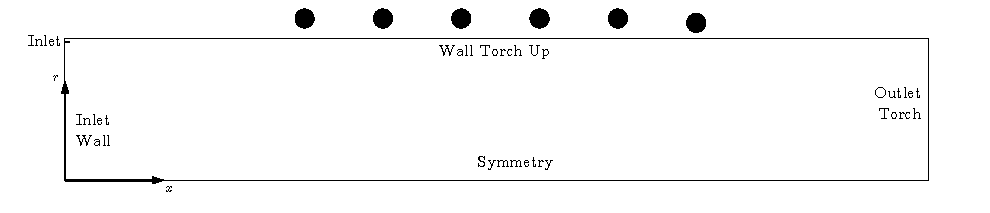
\includegraphics[width=\textwidth]{geom_torch.pdf}
\caption{Geometry of the torch}\label{fig:geomtorch}
\end{figure}
Then, we obtain the same kind of mesh as dawned in figure \ref{fig:meshtorch}.
\begin{figure}[hbp]
  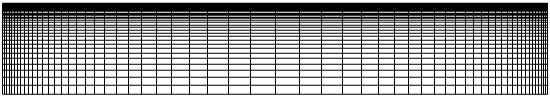
\includegraphics[width=\textwidth]{mesh_torch_3.png}
  \caption{Mesh of the torch}\label{fig:meshtorch}
\end{figure}

This simulation requires the following libraries: 
\begin{verbatim}
Simulator.Modules.Libs = libPetsc libTecplotWriter libNavierStokes libMutation libMutationI \
 libICP libLTE libICPLTE libFiniteVolume libFiniteVolumeNavierStokes libFiniteVolumeICP \
 libNewtonMethod libGambit2CFmesh libCFmeshFileReader libCFmeshFileWriter
\end{verbatim}

\subsection{Physical model}
In the chamber of the Plasmatron the flow can be considered in Local Thermodynamic Equilibrium (LTE). Even though this
hypothesis is not really valid in the torch, it is the model which will give the best solution in the chamber. 
The physical model uses the following options:
\begin{verbatim}
Simulator.SubSystem.Default.PhysicalModelType = ICPLTE2D
Simulator.SubSystem.ICPLTE2D.refValues = 1. 100. 100. 10000. 0.01 0.01 
Simulator.SubSystem.ICPLTE2D.refLength = 1.
Simulator.SubSystem.ICPLTE2D.ConvTerm.uInf = 100.
Simulator.SubSystem.ICPLTE2D.ConvTerm.p0Inf = 10000.
\end{verbatim}
The reference values are used to compute the Jacobian of the linear solver.
\texttt{uInf} and \texttt{p0Inf} are the velocity and the static pressure of the jet. 
Usually, since the velocity is rather small, the flow is considered as incompressible, 
meaning that we do not solve $P$ but its perturbations $\delta P$.

To characterise the model used to compute the magnetic field the following options are used:
\begin{verbatim}
Simulator.SubSystem.ICPLTE2D.SourceTerm.Use2DModel = true
\end{verbatim}
This option give the opportunity to use a simplified 1D model. \\
{\bf WATCH OUT:} In the torch both models can be used, but when the chamber is also considered,
2D effects are no more negligible and {\bf must} be included.\\

To characterize the electric current the following options should be used:
\begin{verbatim}
Simulator.SubSystem.ICPLTE2D.SourceTerm.Permeability = 0.0000012566
Simulator.SubSystem.ICPLTE2D.SourceTerm.Freq = 0.37
\end{verbatim}
The electro-magnetic field can be saved in a file: 
\begin{verbatim}
Simulator.SubSystem.ICPLTE2D.SourceTerm.OutputFile = ./EM.plt
Simulator.SubSystem.ICPLTE2D.SourceTerm.OutputFileSaveRate = 5
\end{verbatim}

The following option add some more messages after a specified number of iterations 
(put 0 in case no extra messages are wanted):
\begin{verbatim}
Simulator.SubSystem.ICPLTE2D.SourceTerm.extraVerboseRate = 10
\end{verbatim}
The following setting ensures compatibility with old FORTRAN ICP code, using a 
correction ($\sigma = 904.11 + (\sigma-904.11)*0.91)$) for the 
electrical conductivity $\sigma$ for $T>7250$ [K]:
\begin{verbatim}
Simulator.SubSystem.ICPLTE2D.SourceTerm.PegaseApproximation = true
\end{verbatim}

Then we define the chemical library that will take care of providing the 
thermodynamic, chemical and transport properties of the real gas. 
This library is MUTATION:
\begin{verbatim}
 Simulator.SubSystem.ICPLTE2D.PropertyLibrary = Mutation
\end{verbatim}
It is possible to choose which mixture to use (argon, air, $CO_2$). 
Moreover, several mixtures for air (air with 5, 7, or 11 species) are available.
\begin{verbatim}
 Simulator.SubSystem.ICPLTE2D.Mutation.mixtureName = air11
\end{verbatim}

\begin{verbatim}
Simulator.SubSystem.ICPLTE2D.Mutation.thermCondAlgo = Direct
\end{verbatim}
specifies to use a direct transport algorithm for computing the thermal conductivity.

\subsection{Finite Volume solver}

Here we use a cell centered Finite Volume solver where the jacobian is computed numerically.
The following standard settings for the implicit Finite Volume solver should not be changed:

\begin{verbatim}
Simulator.SubSystem.SpaceMethod = CellCenterFVM
Simulator.SubSystem.CellCenterFVM.Data.CollaboratorNames = NSLSS ELSS
Simulator.SubSystem.CellCenterFVM.ComputeRHS = NumJacobCoupling
Simulator.SubSystem.CellCenterFVM.NumJacobCoupling.FreezeDiffCoeff = false
\end{verbatim}

The following options specify to use a pseudo-steady time-dependent residual, 
where the time dependent part of the implicit flux jacobian for the two 
magnetic induction equations (second system of equations) is annulled 
(i.e., set to 0), while the corresponding term is kept for the 
hydrodynamic equations (first system). This treatment improves convergence.
\begin{verbatim}
Simulator.SubSystem.CellCenterFVM.ComputeTimeRHS = PseudoSteadyTimeRhsCoupling
Simulator.SubSystem.CellCenterFVM.PseudoSteadyTimeRhsCoupling.annullDiagValue = 0 1
\end{verbatim}

The Rhie-Chow flux splitter is used for computing the convective part of an
incompressible flow:
\begin{verbatim}
Simulator.SubSystem.CellCenterFVM.Data.FluxSplitter = RhieChow2D
Simulator.SubSystem.CellCenterFVM.Data.RhieChow2D.PressStab = false
Simulator.SubSystem.CellCenterFVM.Data.RhieChow2D.PressDissipScale = 1.
\end{verbatim}

The solution is updated at each pseudo-time iteration in [dp, u, v, T], while the equations are formulated 
in conservative variables. The diffusive term is also computed starting from [dp, u, v, T].
\begin{verbatim}
Simulator.SubSystem.CellCenterFVM.Data.UpdateVar  = Puvt
Simulator.SubSystem.CellCenterFVM.Data.SolutionVar = Cons 
Simulator.SubSystem.CellCenterFVM.Data.DiffusiveVar = Puvt
\end{verbatim}

The viscous term is computed by the following diffusive flux
\begin{verbatim}
Simulator.SubSystem.CellCenterFVM.Data.DiffusiveFlux = NavierStokesCoupling
\end{verbatim}
Four source terms are used: one due to the axi-symmetry, one due to the Joule effect, the Lorentz force
caused by the magnetic field and one due to the magnetic induction:
\begin{verbatim}
Simulator.SubSystem.CellCenterFVM.Data.isAxisymm = true
Simulator.SubSystem.CellCenterFVM.Data.SourceTerm = \
 NavierStokesIncomp2DAxiST ICPIncompInductionEquationST
 RMSJouleHeatST LorentzForceAlternativeST
\end{verbatim}

The coupling between the equations through the source term needs some preprocessing:
\begin{verbatim}
Simulator.SubSystem.DataPreProcessing = DataProcessing
Simulator.SubSystem.DataProcessing.Data.updateVar = Puvt
Simulator.SubSystem.DataProcessing.Comds = RMSJouleHeatSourceCoupling \
                                           LorentzForceSourceTermComm
Simulator.SubSystem.DataProcessing.Names = JouleHeatSource LorentzForce
Simulator.SubSystem.DataProcessing.ProcessRate = 1
\end{verbatim}

\subsubsection{Polynomial reconstruction}

The following options should be kept frozen:

\begin{verbatim}
Simulator.SubSystem.CellCenterFVM.SetupCom = LeastSquareP1Setup
Simulator.SubSystem.CellCenterFVM.SetupNames = Setup1
Simulator.SubSystem.CellCenterFVM.Setup1.stencil = FaceVertexPlusGhost
Simulator.SubSystem.CellCenterFVM.UnSetupCom = LeastSquareP1UnSetup
Simulator.SubSystem.CellCenterFVM.UnSetupNames = UnSetup1
Simulator.SubSystem.CellCenterFVM.Data.PolyRec = LinearLS2D

# the following settings of the flux limiter can be commented out in first order
# simulations, but are needed in second order
Simulator.SubSystem.CellCenterFVM.Data.Limiter = Venktn2D
Simulator.SubSystem.CellCenterFVM.Data.Venktn2D.coeffEps = 1.0
Simulator.SubSystem.CellCenterFVM.Data.Venktn2D.useFullStencil = true
# set true the following for backward compatibility, but false should behave better
Simulator.SubSystem.CellCenterFVM.Data.Venktn2D.useNodalExtrapolationStencil = false
Simulator.SubSystem.CellCenterFVM.Data.Venktn2D.length = 1.0
\end{verbatim}

The following factor determines if the simulation is of first, second or in-between order:
\begin{verbatim}
# 0 <= gradientFactor <= 1, with  0. (first order), 1. (second order)
Simulator.SubSystem.CellCenterFVM.Data.LinearLS2D.gradientFactor = 0.
\end{verbatim}
This is an interactive parameter that can be placed into the interactive file. Another interactive parameter,
important for second order computations, is 

\begin{verbatim}
Simulator.SubSystem.CellCenterFVM.Data.LinearLS2D.limitRes = -15.0
\end{verbatim}
This corresponds to the minimum residual at which the freezing of the flux limiter should be applied for flows exhibiting 
discontinuities or steep gradients (e.g., in temperature). In practice, {\tt limitRes} can be kept at  $-15$ till when 
the simulation reaches a limit cycle and then can be increased to $8.$ in order to exit the cycle. This cure is not 
always effective and it often depends on the moment when {\tt limitRes} is increased.\\
{\bf WATCH OUT:} {\it Before restarting a simulation from a second order solution, if the limiter has not been explicitly saved in the CFmesh file 
  (see below), {\tt limitRes} has to be set back to $-15$.}

In order to save the limiter in second order calculations (when {\tt gradientFactor = 1.}), the following options must be added to the CFcase {\bf before} 
starting the computation:

\begin{verbatim}
Simulator.SubSystem.CFmesh.Data.ExtraStateVarNames = limiter

# the following must be the total number of equations
Simulator.SubSystem.CFmesh.Data.ExtraStateVarStrides = 6
\end{verbatim}

Finally, in order to restart from a file in which the limiter {\bf has been already saved}, 
the following line should be included in the CFcase file:

\begin{verbatim}
Simulator.SubSystem.CFmeshFileReader.Data.ExtraStateVarNames = InitLimiter
\end{verbatim}

{\bf WATCH OUT:} {\it When starting from scratch or for very stiff problems, use first order:
\begin{verbatim}
Simulator.SubSystem.CellCenterFVM.Data.LinearLS2D.gradientFactor = 0.
\end{verbatim}
  
  Alternatively, an obsolete way of imposing first order consists in replacing {\tt LinearLS2D} with {\tt Constant}:

\begin{verbatim}
  Simulator.SubSystem.CellCenterFVM.Data.PolyRec = Constant
\end{verbatim}
}

% #-------------------------------------------------------------------------------------
% #-------------------------------------------------------------------------------------
% ####### USER INPUTS ##################################################################
% #-------------------------------------------------------------------------------------
% #-------------------------------------------------------------------------------------
% 
% # directory from which reading inputs and where this CFcase file is located
% Simulator.Paths.WorkingDir = ./
% 
% # directory where ouput files are written
% Simulator.Paths.ResultsDir = ./OUTPUT
% 

\subsection{Stop condition}
There are several ways to define the criteria to stop the simulation:
\begin{itemize}
 \item It is possible to prescribe a maximum number of iterations:
\begin{verbatim} 
Simulator.SubSystem.StopCondition          = MaxNumberSteps
Simulator.SubSystem.MaxNumberSteps.nbSteps = 4
\end{verbatim}
\item It is also possible to stop the simulation when the residual (which is an indicator of the error)
reaches a threshold value:
\begin{verbatim}
Simulator.SubSystem.StopCondition       = Norm
Simulator.SubSystem.Norm.valueNorm      = -2.0
\end{verbatim}
\end{itemize}
Actually, in this phase of the simulation where there are not yet the full coupling with the electro-magnetism,
we do not want to get a very small residual. We just want to start to converge the flow field. This phase should not be long
(around 500-1500 iterations).
The simulation should be manually stopped when the flow field and the temperature look like in the next plot.
\begin{figure}[htbp]
 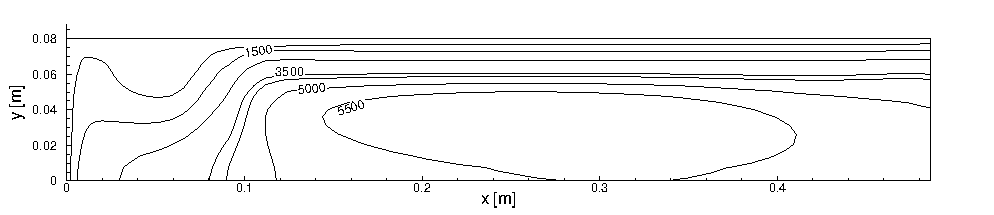
\includegraphics[width=\textwidth]{torch_T_nc.pdf}
\caption{Temperature iso-lines}\label{fig:}
\end{figure}
\begin{figure}[hbp]
 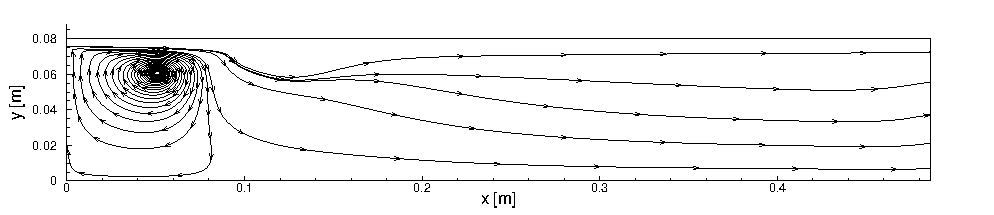
\includegraphics[width=\textwidth]{torch_SL_nc.pdf}
\caption{Streamlines in the torch at the end of the first phase}\label{fig:}
\end{figure}

\subsection{Importing the mesh}
It is important to define the list of the names of the TRS (topological region surface), which
correspond to the list of the names of the boundaries. If you start from a gambit file they are listed at
the end of the file.
\begin{verbatim}
 Simulator.SubSystem.Default.listTRS = \
   Symmetry Wall_torch_up Wall_torch_in Inlet Outlet_torch 
\end{verbatim}
Then you give the name of the mesh file
\begin{verbatim}
Simulator.SubSystem.CFmeshFileReader.Data.FileName = torch_4.CFmesh
\end{verbatim}
{\bf WATCH OUT:} The file name should always be with the CFmesh extension, even 
if the mesh file is from Gambit

To load and read the mesh the following options should be used
\begin{verbatim}
Simulator.SubSystem.MeshCreator = CFmeshFileReader
Simulator.SubSystem.CFmeshFileReader.convertFrom = Gambit2CFmesh
Simulator.SubSystem.CFmeshFileReader.Gambit2CFmesh.Discontinuous = true
Simulator.SubSystem.CFmeshFileReader.Gambit2CFmesh.SolutionOrder = P0
Simulator.SubSystem.CFmeshFileReader.Data.ScalingFactor = 1000
\end{verbatim}
The option \texttt{ScalingFactor} corresponds to the factor that should be used
to divide the gambit mesh in order to obtain the right geometry.\\
The following settings should only be activated (uncommented) when starting a ICP simulation from a 
pure hydrodynamic field, i.e., from a CFmesh file with only [dp u v T], without 
magnetic field data. In this case, during the restart, ER and EI are initialized to 0.
 
\begin{verbatim}
#Simulator.SubSystem.CFmeshFileReader.Data.UseInitValues = 0 0 0 0 1 1 
#Simulator.SubSystem.CFmeshFileReader.Data.InitValues = 0. 0. 0. 0. 0. 0. 
\end{verbatim}

\subsection{Writing outputs}
It is possible to write solution files in CFmesh, tecplot, paraview....
\begin{verbatim}
Simulator.SubSystem.OutputFormat        = Tecplot CFmesh
\end{verbatim}
It is also possible to specify which variables we want in the solution.
Here we will have the pressure perturbations, the velocity and the temperature. 
\begin{verbatim}
 Simulator.SubSystem.Tecplot.Data.outputVar = Puvt
\end{verbatim}
It is also useful to be able to visualize extra variables such as the Mach, the enthalpy, the total temperature and pressure....
\begin{verbatim}
Simulator.SubSystem.Tecplot.Data.printExtraValues = true
\end{verbatim}
The options to set the frequency of saving and the name files are as follows:
\begin{verbatim}
 Simulator.SubSystem.CFmesh.FileName     = torch_4-out.CFmesh
 Simulator.SubSystem.CFmesh.SaveRate     = 50
 Simulator.SubSystem.CFmesh.AppendIter   = true
 
 Simulator.SubSystem.Tecplot.FileName    = torch_4-out.plt
 Simulator.SubSystem.Tecplot.SaveRate    = 50 
\end{verbatim}
It is also possible to write the solution for a particular TRS:
\begin{verbatim}
Simulator.SubSystem.Tecplot.Data.SurfaceTRS = Wall_torch_in
\end{verbatim}

\subsection{Pseudo-time discretisation}
We use an implicit discretisation of the pseudo-time. This means
that the pseudo-time component is discretised by a backward Euler:
$$\frac{u^{n+1}-u^n}{\Delta \tau} = R(u^{n+1})$$
The system obtained is solved by a GMRES algorithm provided by 
an external library called PETSC. Here two solvers are used: one for dp, u, v, T
and the other for the electromagnetic field (which corresponds to variables 4 and 5)
\begin{verbatim} 
Simulator.SubSystem.LinearSystemSolver = PETSC PETSC
Simulator.SubSystem.LSSNames = NSLSS ELSS

Simulator.SubSystem.NSLSS.Data.PCType = PCASM
Simulator.SubSystem.NSLSS.Data.KSPType = KSPGMRES
Simulator.SubSystem.NSLSS.Data.MatOrderingType = MATORDERING_RCM
Simulator.SubSystem.NSLSS.Data.MaxIter = 1000
Simulator.SubSystem.NSLSS.MaskEquationIDs = 0 1 2 3
Simulator.SubSystem.NSLSS.Data.NbKrylovSpaces = 50
Simulator.SubSystem.NSLSS.Data.RelativeTolerance = 1e-4

Simulator.SubSystem.ELSS.Data.PCType = PCASM
Simulator.SubSystem.ELSS.Data.KSPType = KSPGMRES
Simulator.SubSystem.ELSS.Data.MatOrderingType = MATORDERING_RCM
Simulator.SubSystem.ELSS.Data.MaxIter = 100
Simulator.SubSystem.ELSS.MaskEquationIDs = 4 5
Simulator.SubSystem.ELSS.Data.NbKrylovSpaces = 80
Simulator.SubSystem.ELSS.Data.RelativeTolerance = 1e-4
\end{verbatim}

{\tt MaxIter} defines the maximum allowed number of GMRES iterations and 
should be kept $<= 1000$. {\tt RelativeTolerance} defines the relative tolerance for the GMRES solver: $1e-4$ or $1e-3$ are recommended values, since with higher values 
convergence can be very slow and requiring many more GMRES iterations per time step. \\
The coupling between the Backward Euler and PETSC (which is called NewtonIterator) is defined as follows :
\begin{verbatim}
Simulator.SubSystem.ConvergenceMethod = NewtonIterator
Simulator.SubSystem.NewtonIterator.AbsoluteNormAndMaxIter.MaxIter = 1
Simulator.SubSystem.NewtonIterator.ConvRate = 1
Simulator.SubSystem.NewtonIterator.ShowRate = 1
Simulator.SubSystem.NewtonIterator.Data.CollaboratorNames = NSLSS ELSS
\end{verbatim}
It is possible to choose which variable will be used to check the convergence criteria
to stop the iterations:
\begin{verbatim}
Simulator.SubSystem.NewtonIterator.Data.L2.MonitoredVarID = 0
\end{verbatim}

The update of the solution can be under-relaxed so that ${\bf U}^{n+1} = {\bf U}^{n} + {\bf \alpha}*{\bf \delta U}$
where ${\bf \alpha}$ is an array of values (one per all or one per variable), as specified by 
\begin{verbatim}
Simulator.SubSystem.NewtonIterator.StdUpdateSol.Relaxation = .3 .3 .3 .3 1. 1.
\end{verbatim}

\subsection{CFL}
To define the CFL (which will mainly correspond to the ratio between $\Delta \tau$ and $\Delta x$)\\
Several ways to define it are available:
\begin{itemize}
\item By a constant value
\begin{verbatim}
Simulator.SubSystem.NewtonIterator.Data.CFL.Value = 0.1
\end{verbatim}
\item By a function:
\begin{verbatim}
Simulator.SubSystem.NewtonIterator.Data.CFL.Value = 0.1
Simulator.SubSystem.NewtonIterator.Data.CFL.ComputeCFL = Function 
Simulator.SubSystem.NewtonIterator.Data.CFL.Function.Def = 
                           if(i>100,min(10,cfl*1.05),0.1)
\end{verbatim}
{\bf WATCH OUT:} Even if a function is used it is necessary to fill the option \texttt{Value} which
 will be used for the first iteration.

\item In this test case the best, is to use an interactive CFL
\begin{verbatim}
 Simulator.SubSystem.NewtonIterator.Data.CFL.ComputeCFL = Interactive
 Simulator.SubSystem.NewtonIterator.Data.CFL.Interactive.CFL = 0.0001
 Simulator.SubSystem.InteractiveParamReader.FileName = ./torch.inter
 Simulator.SubSystem.InteractiveParamReader.readRate = 5
\end{verbatim}
The interactive file will be read every 5 iterations. It should look like
\begin{verbatim}
Simulator.SubSystem.NewtonIterator.Data.CFL.Interactive.CFL = 0.0001
\end{verbatim}
In the initial phase of the simulation (if starting from scratch), 
the CFL should be extremely small and should not change much.
\end{itemize}

Since flow solution is computed in the cell centers, nodal values must be extrapolated from cell centers 
to the mesh vertices for visualization purposes or for computing viscous gradients. This is accomplished by 
{\tt NodalExtrapolation} objects. In viscous cases, where a slip condition and, possibly, a temperature 
are imposed at the wall, the following settings must be added in order to strongly impose the desired values.

\begin{verbatim}
# nodal conditions on TRS's for which some variables have to imposed strongly 
# .ValuesIdx specifies IDs of the variables to impose
# .Values    specifies value for the corresponding variable to impose
Simulator.SubSystem.CellCenterFVM.Data.NodalExtrapolation = DistanceBasedGMoveMultiTRS

# order of application of BCs (this determines which condition to impose in corners)
Simulator.SubSystem.CellCenterFVM.Data.DistanceBasedGMoveMultiTRS.TrsPriorityList = \
 	Wall_torch_up Symmetry Wall_torch_in Inlet Outlet_torch

# names of the boundary patches (TRS) on which a some values will be forced strongly
Simulator.SubSystem.CellCenterFVM.Data.DistanceBasedGMoveMultiTRS.TRSName = \
         Wall_torch_up Symmetry Wall_torch_in Inlet

# each boundary treatment, one by one, is specified here after

# u, v, T are imposed on the boundary vertices on the torch upper wall
Simulator.SubSystem.CellCenterFVM.Data.
         DistanceBasedGMoveMultiTRS.Wall_torch_up.ValuesIdx = 1 2 3     
Simulator.SubSystem.CellCenterFVM.Data.
         DistanceBasedGMoveMultiTRS.Wall_torch_up.Values = 0. 0. 350. 
 
# ER, EI are imposed to 0 on the symmetry axis
Simulator.SubSystem.CellCenterFVM.Data.
         DistanceBasedGMoveMultiTRS.Symmetry.ValuesIdx = 4 5    
Simulator.SubSystem.CellCenterFVM.Data.
         DistanceBasedGMoveMultiTRS.Symmetry.Values = 0. 0.

# u, v, T, ER, EI are imposed on the boundary wall at the torch inlet
Simulator.SubSystem.CellCenterFVM.Data.
         DistanceBasedGMoveMultiTRS.Wall_torch_in.ValuesIdx = 1 2 3 4 5 
Simulator.SubSystem.CellCenterFVM.Data.
         DistanceBasedGMoveMultiTRS.Wall_torch_in.Values = 0. 0. 350. 0. 0.

# T, ER, EI are imposed at the torch inlet
Simulator.SubSystem.CellCenterFVM.Data.
         DistanceBasedGMoveMultiTRS.Inlet.ValuesIdx = 3 4 5
Simulator.SubSystem.CellCenterFVM.Data.
         DistanceBasedGMoveMultiTRS.Inlet.Values = 350. 0. 0.

# p, ER, EI are imposed at the outlet of the torch
Simulator.SubSystem.CellCenterFVM.Data.
         DistanceBasedGMoveMultiTRS.Outlet_torch.ValuesIdx = 0 4 5
Simulator.SubSystem.CellCenterFVM.Data.
         DistanceBasedGMoveMultiTRS.Outlet_torch.Values = 0. 0. 0.
\end{verbatim}

\subsection{Initialization}
In this first phase the solution is initialized by a very rough estimation of what would look like the velocity field and the 
temperature in the torch. This will considerably help the convergence. For instance, the temperature will be set as plotted in figure \ref{fig:inittorch}.
\begin{figure}[htbp]
 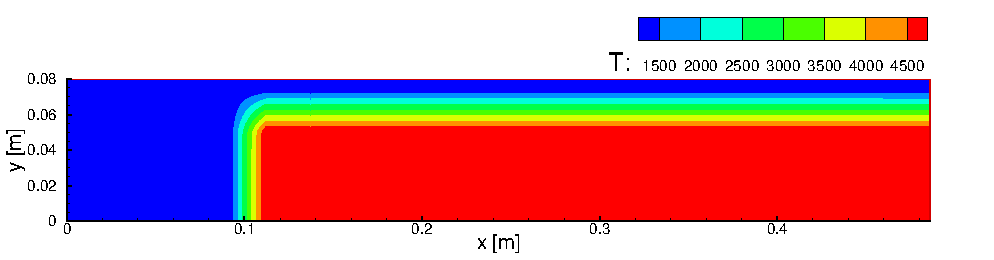
\includegraphics[width=\textwidth]{torch_T_initial.pdf}
\caption{Temperature iso-lines of the initial solution}\label{fig:inittorch}
\end{figure}
The option needs to be defined as follows:
\begin{verbatim}
Simulator.SubSystem.CellCenterFVM.InitComds = InitState
Simulator.SubSystem.CellCenterFVM.InitNames = InField
Simulator.SubSystem.CellCenterFVM.InField.applyTRS = InnerFaces
Simulator.SubSystem.CellCenterFVM.InField.Vars = x y
Simulator.SubSystem.CellCenterFVM.InField.Def = 
                    0. \
                    if(y>.075,if(y<.08,100.,0.),if(x>.2,0.,0.)) \
                    0. \
                    if(x>0.1,if(y>.075,1000.,if(y>.05,-(4000./.025)*
                       (y-.05)+5000.,5000.)),1000.) \
                    0. \
                    0.
\end{verbatim}

\subsection{Boundaries conditions}
In this phase, the boundary conditions are not imposing any coupling with the magnetic field. 
In the following, a list of boundary conditions for the Navier-Stokes equation system is presented following the notation of figure \ref{fig:geomtorch}:
\begin{itemize}
\item \textbf{Inlet}(\texttt{SubInletICP2DPuvtUVTFVMCC}). The inlet is placed in the left boundary, and spans from $r=75 mm$ to $r=80 mm$, which corresponds to the upper wall. The chosen inlet gas model is \emph{air11},
 and its thermodynamic conditions have to be set as well. Usually the static pressure will be set to $10000Pa$ and the temperature of the air to $350K$. The mass flow must be imposed as well, 
and for this project we will work with a $16g/s$ mass flow.
\item \textbf{Inlet wall}(\texttt{NoSlipWallIsothermalICPPvtFVMCC}). On this edge the no-slip condition is applied. This is the boundary that produces most of the convergence problems. Usually, we impose a constant temperature on this wall,
 but during this project we choose an adiabatic wall in order to avoid convergence problems with the second order schemes. A deeper analysis of the influence of the boundary condition on this part  of the domain can be found in Section \ref{sec:torch_remarks}. Briefly, the adiabatic wall will imposes a temperature gradient equal to zero at the wall; in other words, no heat transfer will be
 produced. 
\item \textbf{Wall torch up}(\texttt{NoSlipWallIsothermalICPPvtFVMCC}). This wall is set to isothermal, and the selected temperature is $350K$, the same temperature as the inlet gas. Of course, the no-slip condition is also imposed along
 the edge. One should not expect any problem from this boundary since the flow in the vicinity will remain at low temperature.
\item \textbf{Symmetry} (\texttt{MirrorICPFVMCC}). Provided that the problem is axisymmetric, in this boundary all the radial gradients will be equal to zero. Moreover, the symmetry of the problem implies that the vertical
 velocity will be zero as well on the axis.
\item \textbf{Outlet}(\texttt{SubOutletICP2DPuvtFVMCC}). Since the Mach number is expected to be very low ($\sim 0.2$), the outlet of the torch will be set to subsonic. Hence, the static pressure is imposed to $10000Pa$.
\end{itemize}
To impose this with COOLFLuiD, you should first define the list of commands:
\begin{verbatim}
Simulator.SubSystem.CellCenterFVM.BcComds = NoSlipWallIsothermalICPPvtFVMCC \
                                             MirrorICPFVMCC \
                                             NoSlipWallIsothermalICPPvtFVMCC \
                                             SubInletICP2DPuvtUVTFVMCC \
                                             SubOutletICP2DPuvtFVMCC 
\end{verbatim} 
Then, you give a name to each boundary conditions:
\begin{verbatim}
Simulator.SubSystem.CellCenterFVM.BcNames = BcTorchWallUp \
                                            BcSymmetry \
                                            BcTorchWallIn \
                                            BcInlet \
                                            BcOutletTorch
\end{verbatim}

And then, we define the options:
\begin{itemize}
 \item At the outlet we impose a constant pressure. Since the flow is incompressible,
we are not solving the pressure but its perturbations, that is why we impose zero.
\begin{verbatim}
 Simulator.SubSystem.CellCenterFVM.BcOutletTorch.applyTRS = Outlet_torch
 Simulator.SubSystem.CellCenterFVM.BcOutletTorch.P = 0.0
\end{verbatim}
\item For the walls it is only necessary to impose a constant temperature which is around 350K in the Plasmatron
\begin{verbatim}
  Simulator.SubSystem.CellCenterFVM.BcTorchWallUp.applyTRS = Wall_torch_up
  Simulator.SubSystem.CellCenterFVM.BcTorchWallUp.TWall = 350.

  Simulator.SubSystem.CellCenterFVM.BcTorchWallIn.applyTRS = Wall_torch_in
  Simulator.SubSystem.CellCenterFVM.BcTorchWallIn.TWall = 350.
\end{verbatim}
\item At the inlet we need to impose the mass flow, the temperature and to define
the internal and external radius of the jet.
\begin{verbatim}
 Simulator.SubSystem.CellCenterFVM.BcInlet.applyTRS = Inlet
 Simulator.SubSystem.CellCenterFVM.BcInlet.MassFlow = 16.
 Simulator.SubSystem.CellCenterFVM.BcInlet.T = 350.
 Simulator.SubSystem.CellCenterFVM.BcInlet.InletRadii = .075 .08
\end{verbatim}
\item In the case of the symmetry axis there are no options to define
\begin{verbatim}
 Simulator.SubSystem.CellCenterFVM.BcSymmetry.applyTRS = Symmetry
\end{verbatim}
\end{itemize}
\subsection{Setup of the coils, current, power and Lorentz forces}
The plasma power is defined as follows
\begin{verbatim}
 Simulator.SubSystem.DataProcessing.JouleHeatSource.DesiredPower = 90.
\end{verbatim}
{\bf WATCH OUT:} This is the plasma power and not the generator power. The efficiency of the
generator is around 0.5 (to check with Olivier and Francesco)
The position, radius and number of coils is set up as follows:
\begin{verbatim}
 Simulator.SubSystem.DataProcessing.JouleHeatSource.DesiredPower = 90.
 Simulator.SubSystem.DataProcessing.JouleHeatSource.NbCoils = 6
 Simulator.SubSystem.DataProcessing.JouleHeatSource.RadiusCoils = .109 .109 .109 \
                                                                  .109 .109 .109
 Simulator.SubSystem.DataProcessing.JouleHeatSource.ZPositionCoils = .127 .177 .227 \
                                                                     .277 .327 .377
\end{verbatim}
It is possible to save the current field in a file:
\begin{verbatim}
  Simulator.SubSystem.DataProcessing.JouleHeatSource.OutputFileElCurrent = ./elCurrent.plt
\end{verbatim}


There are several possibilities to compute the electric field E for the Lorentz force
\begin{itemize}
 \item 0: E in the middle of the face obtained from E in adjacent nodes 
 \item 1: E in the middle of the face obtained with complete distance-base diamond-shape stencil (DEFAULT)
 \item 2: E in the middle of the face obtained from E in cell centers
\end{itemize}
The way to set it:
\begin{verbatim}
 Simulator.SubSystem.DataProcessing.LorentzForce.FaceCenterComputationMethod = 1
\end{verbatim}

There are also several ways to compute the average of the electric field Ev:
\begin{itemize}
 \item 0: LorentzForce takes computed Ev coming from RMSJouleHeatSourceComm.cxx (DEFAULT)
 \item 1: LorentzForce compute Ev usign distance-based average 
 \item 2: LorentzForce computes Ev in the original way, using volume-based average
\end{itemize}
This is defined by:
\begin{verbatim}
 Simulator.SubSystem.DataProcessing.LorentzForce.AverageInNodeStrategy = 0
\end{verbatim}

\section{Full torch}
Now, we will add the coupling between the flow field and the electromagnetism though the boundaries. So,
we restart from the solution file (.CFmesh) of the previous simulation.
The difference in the CFcase between the phase one and two, concerns the importation of the mesh, the definition
of the CFL and priority of the boundary conditions.

\subsection{Reading of the mesh and initial condition}
Now, the option to load the solution should be 
\begin{verbatim}
Simulator.SubSystem.Default.listTRS = InnerFaces Symmetry Wall_torch_up Wall_torch_in
                                  Inlet Outlet_torch
Simulator.SubSystem.MeshCreator = CFmeshFileReader
Simulator.SubSystem.CFmeshFileReader.Data.FileName = torch_4-out-P1.CFmesh
\end{verbatim}
It is also important to fill the option allowing to restart from this solution:
\begin{verbatim}
Simulator.SubSystem.CellCenterFVM.Restart = true
\end{verbatim}

\subsection{CFL law}
In this phase, it is possible to increase much more the CFL (than in the previous phase). The more practical,
is to use a function to define the CFL:
\begin{verbatim}
 Simulator.SubSystem.NewtonIterator.Data.CFL.Value = 0.01
Simulator.SubSystem.NewtonIterator.Data.CFL.ComputeCFL = Function 
Simulator.SubSystem.NewtonIterator.Data.CFL.Function.Def = 
         if(i>80,if(i>105,if(i>130,if(i>160,if(i>200,if(i>225,
                            if(i>245,600,400),120),60),20),10),5),1)
\end{verbatim}
In general the CFL can follow the law defined in table \ref{tab:cfl_torch_fir}.
\begin{table}[htb]
\centering
\begin{tabular}{lc}
\textbf{Iteration} & \textbf{CFL} \\ \hline
$1 \sim 10 $ & 0.01 \\ \hline
$10 \sim 45 $ & 0.1 \\ \hline
$45 \sim 100 $ & 1 \\ \hline
$100 \sim 295 $ & 10 \\ \hline
$>295$ & 100 \\ 
\hline
\end{tabular}
\caption{Example of a CFL law for the first order - restart simulation.}
\label{tab:cfl_torch_fir}
\end{table}

\subsection{Initialisation and boundary conditions}
The initialization is not necessary any more, since we restart from a previous solution.
Concerning the boundary conditions, only the command are changing:
\begin{verbatim}
 Simulator.SubSystem.CellCenterFVM.BcComds = EpComputingNoSlipWallIsothermalICPPvtFVMCC \
                                            MirrorICPFVMCC \
                                            EpComputingNoSlipWallIsothermalICPPvtFVMCC \
                                            EpComputingSubInletICP2DPuvtUVTFVMCC \
                                            EpComputingSubOutletICP2DPuvtFVMCC \
\end{verbatim}


\section{Initialisation of the chamber}

\section{Full gemoetry in 1st order}

\section{Full gemoetry in 2nd order}





\end{document}
